%%%%%%%%%%%%%%%%%%%%%%%%%%%%%%%%%%%%%%%%%%%%%%%%%%%%%%%%%%%%%%%%%
%
% Project     : Turnverein App
% Title       : 
% File        : umsetzung.tex Rev. 00
% Date        : 07.07.14
% Author      : Raffael Santschi
%
%%%%%%%%%%%%%%%%%%%%%%%%%%%%%%%%%%%%%%%%%%%%%%%%%%%%%%%%%%%%%%%%%

\chapter{Umsetzung des Prototyps}\label{chap.umsetzung}
In diesem Kapitel wird kurz auf die Entwicklungsumgebung für dieses Projekt eingegangen. Danach wird erklärt, wie die Umsetzung des Backends und des Mobile App Prototyps durchgeführt wurde.

\section{Entwicklungsumgebung}\label{entwicklungsumgebung}
Ein Softwareprojekt benötigt immer eine gewisse Umgebung, welche die erforderlichen Funktionen erfüllt. Die Entwicklung einer App mit Hilfe von Phonegap kommt jedoch mit wenig aus und die Entwicklungsumgebung ist schnell aufgebaut.

\subsection{IDE - Integrated Development Environment}
Eine \glossarmark{IDE}, um welche man nicht herum kommt, ist XCode. Sie wird benötigt um die App zu paketieren und sie direkt zur Analyse von Apple hochzuladen. Zusätzlich wurde noch Aptana Studio, welches für Webentwicklung ausgelegt ist, verwendet. Hier könnte man aber auf beliebige Alternativen umsteigen und notfalls auch mit einem gewöhnlichen Texteditor arbeiten. Die Vorteile einer \glossarmark{IDE} sind Syntax-Highlighting, -Checking und Autocompletion.

\begin{figure}[h]
\centering
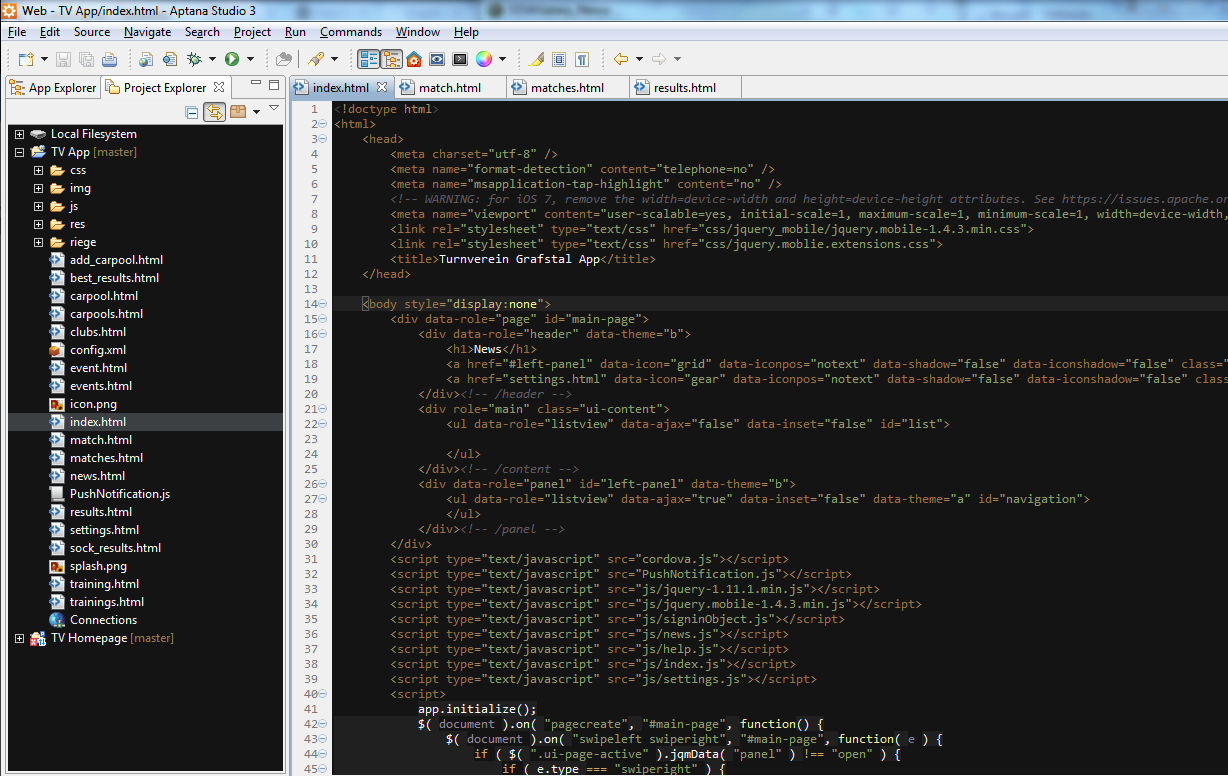
\includegraphics[scale=0.5]{images/aptana.png}
\caption{Aptana Studio}
\label{fig:aptana}
\end{figure}


\subsection{Versionierung}
Versionierung ist in der Softwareentwicklung ein sehr wichtiges Thema, hierzu gibt es verschiedenste Tools, die einen dabei unterstützen. In diesem Projekt wurde git (siehe \cite{git}), was eines der verbreitetsten Versionierungstools ist, verwendet. Das Remote Repository wurde auf Github (siehe \cite{github_app}) erstellt. Es wurde darauf geachtet, dass der Code jeden Abend auf das Repository geladen wurde, damit ein Backup existiert.

\begin{figure}[h]
\centering
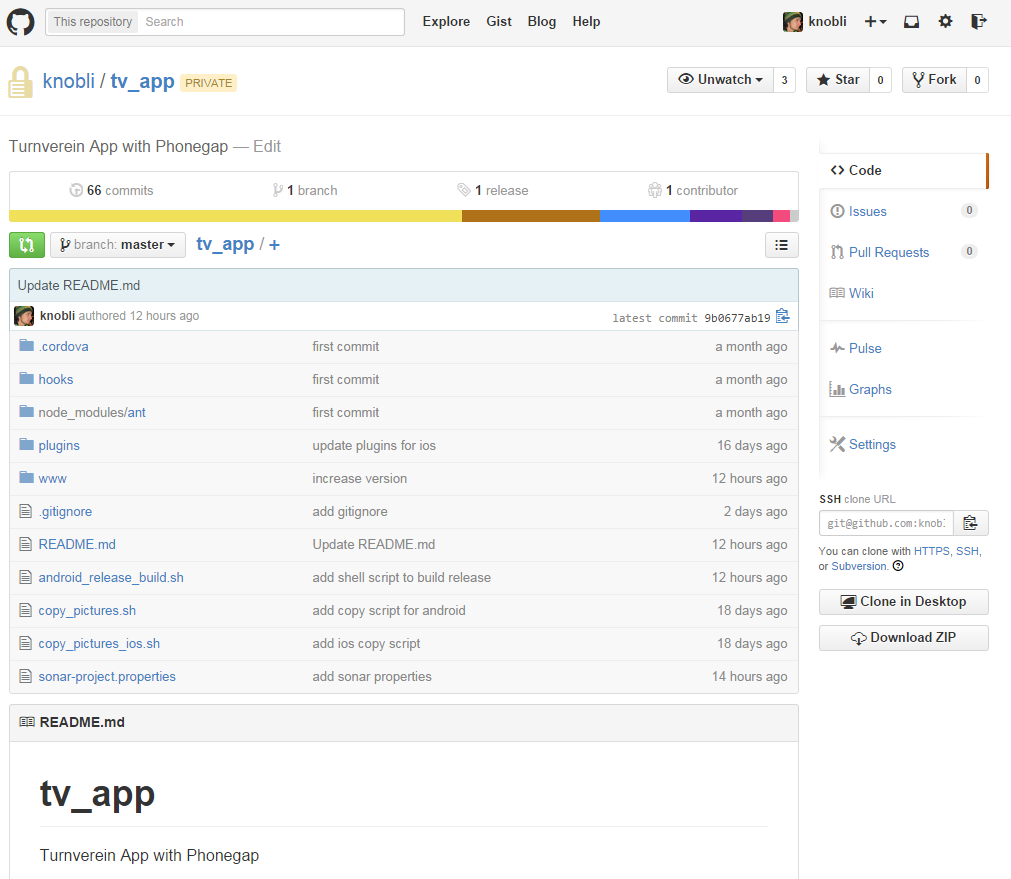
\includegraphics[scale=0.5]{images/github.png}
\caption{Github Repository}
\label{fig:github_repo}
\end{figure}

\newpage
\subsection{SDK - Software Development Kit}
Für die Entwicklung der App auf den beiden Plattformen, Android und iOS, wurden die dazugehörigen SDKs benötigt, um die Applikation in einem Emulator laufen zu lassen. Vor allem bei Android, mit seinen diversen Gerätevariationen, ist dies sinnvoll, da der Emulator jedes beliebige Device emulieren kann.

\begin{figure}[h]
\centering
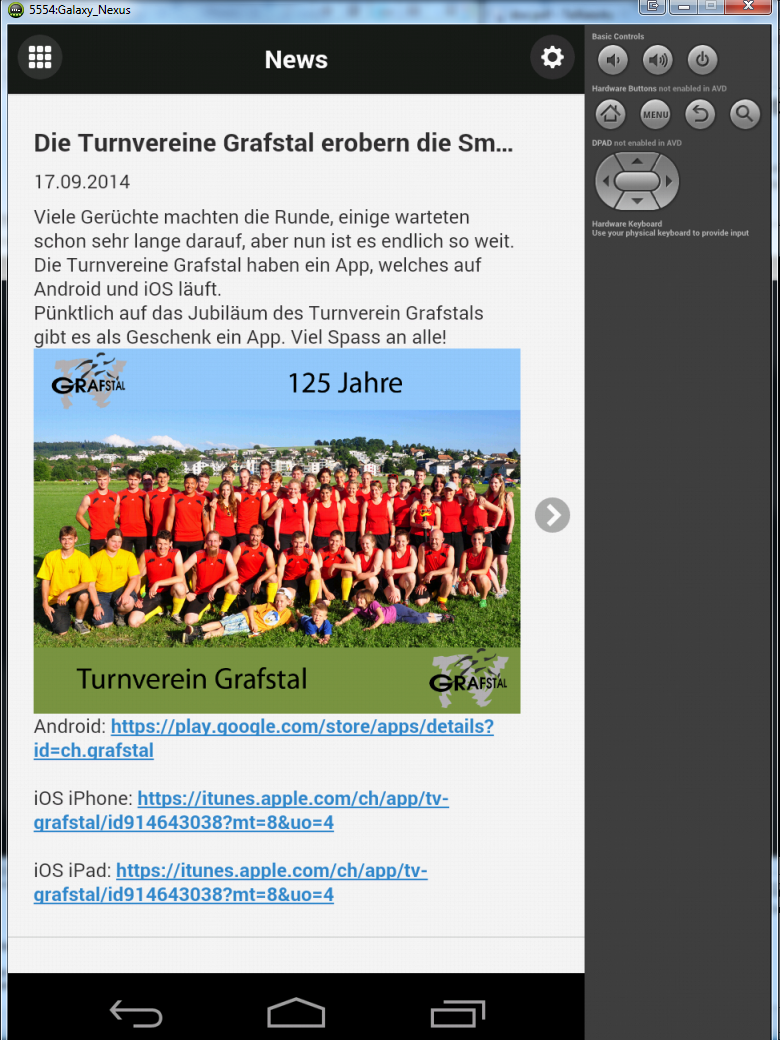
\includegraphics[scale=0.25]{images/android_emulator.png}
\caption{Android Emulator}
\label{fig:android_emulator}
\end{figure}

\FloatBarrier
\subsection{Webbrowser}
Die App wurde nicht nur auf Emulatoren getestet, sondern auch in Browsern. Dazu wurde auf Windows mit Google Chrome und auf Mac OSX mit Safari gearbeitet. Dazu wurde das Backend und die App in einem lokalen Apache Web Server laufen gelassen.

\subsection{Technische Geräte}
Push-Nachrichten können weder auf Emulatoren noch in Webbrowsern getestet werden, dafür benötigt man ein physisches Gerät. Die App wurde auf einem iPhone 4S, iPhone 5S, iPad, Samsung Galaxy Note und Samsung Ace getestet. Für die Entwicklung wurde ein Windows PC verwendet. Damit XCode benutzt werden konnte, wurde zusätzlich noch auf einem iMac gearbeitet.

\newpage
\subsection{Testen - Analysieren}
Zusätzlich zu den manuellen Tests an Geräten und  Emulatoren wurden auch automatisierte Tests und Analysen durchgeführt. Für die automatisierten Tests im Backend wurde PHPunit (siehe \cite{phpunit}) verwendet und für die statische Code Analyse wurde Sonar (siehe \cite{sonar}) mit dem \glossarmark{PHP} und Web Plugin (siehe Abbildung \ref{fig:sonar_backend} und \ref{fig:sonar_app}) aufgesetzt und verwendet. Damit das \glossarmark{API} direkt getestet werden konnte, wurde die Chrome App 'Advanced REST client' (siehe Abbildung \ref{fig:advanced_rest_client}) verwendet.

\begin{figure}[h]
\centering
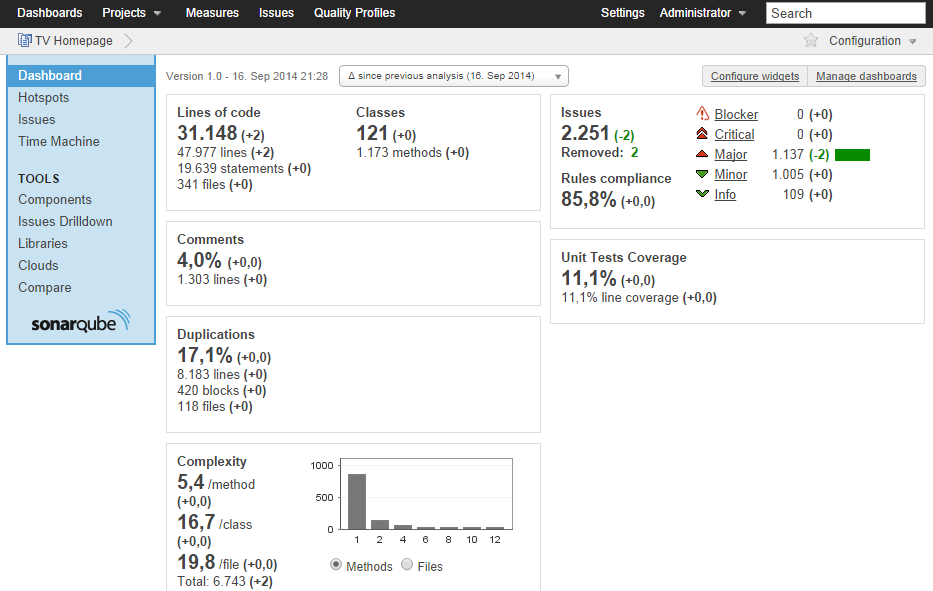
\includegraphics[scale=0.5]{images/sonar_backend.png}
\caption{Sonar - statische Code Analyse Backend}
\label{fig:sonar_backend}
\end{figure}

\begin{figure}[h]
\centering
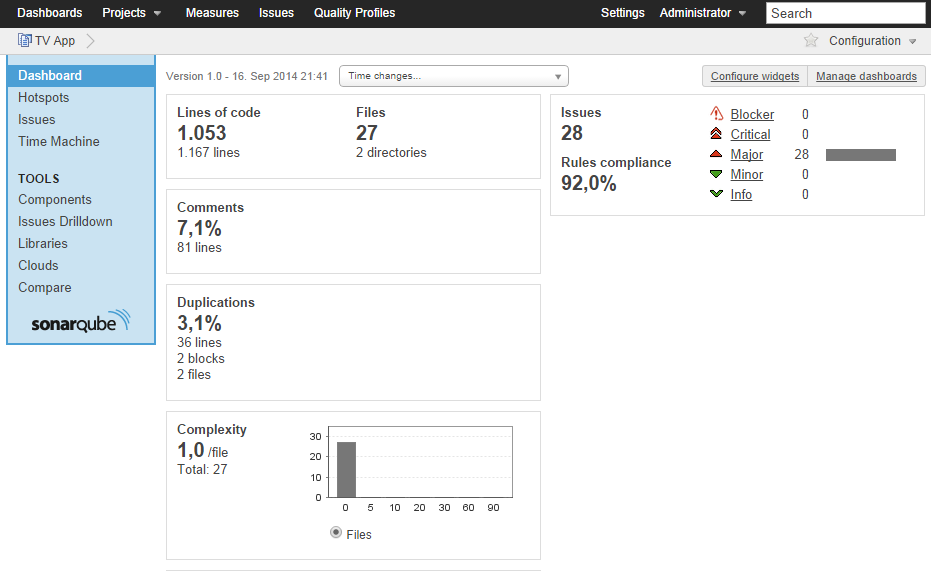
\includegraphics[scale=0.5]{images/sonar_app.png}
\caption{Sonar - statische Code Analyse App}
\label{fig:sonar_app}
\end{figure}

\begin{figure}[h]
\centering
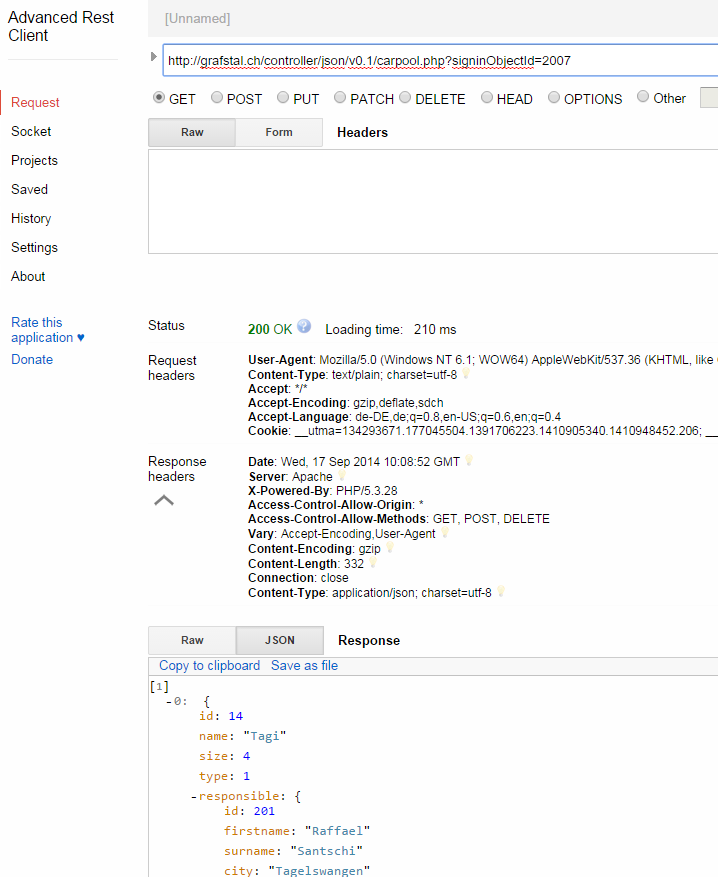
\includegraphics[scale=0.5]{images/advanced_rest_client.png}
\caption{Advanced Rest client}
\label{fig:advanced_rest_client}
\end{figure}

\FloatBarrier


\clearpage
\section{Backend}\label{impl_backend}
In diesem Unterkapitel werden das \glossarmark{Refactoring} des Backends beschrieben und eine Übersicht der Push-Nachricht Implementierung vermittelt.

\subsection{Refactoring}
In diesem Unterkapitel wird kurz der vorgefundene Ist-Zustand beschrieben und danach die Schritte, welche unternommen wurden, um das Backend wartbarer und flexibler zu machen.

\subsubsection{Ist-Zustand}
Zu Beginn dieses Projekts waren in jedem File HTML- mit \glossarmark{PHP}-Code vermischt und SQL-Abfragen waren überall verteilt. Dies erschwerte es erheblich den Code zu warten. Zusätzlich wurde jede save-, update-, load- und delete-Anweisung von Objekten, wenn es denn solche gab, sehr unflexibel selbst implementiert. Zudem erweiterten ähnliche Objekte zwar eine Super-Klasse, teilten sich aber keine Tabelle und hatten somit auch verschiedene ID-Sequenzen.\\

Schnell wurde klar, dass man mit diesem Stand kein \glossarmark{API} aufbauen sollte, welches dann von der App angesprochen wird. Um den Code besser zu strukturieren, übersichtlicher und vor allem auch testbar zu machen, wurde ein \glossarmark{Refactoring} (siehe \cite{feathers2004working}) durchgeführt. Ausgehend von der Strategie für das \glossarmark{Refactoring} wurde Doctrine in das Projekt eingebunden. Doctrine ist, wie schon im Kapitel \ref{arch_backend} erklärt, ein \glossarmark{ORM}, welches, richtig eingesetzt, viel Arbeit abnehmen kann. Damit man Doctrine jedoch sinnvoll verwenden konnte, benötigte es zuerst einige Zeit für die Analyse und die Umstellungen.

\subsubsection{Refactoring}
Zu Beginn wurden mögliche Synergien evaluiert. Alle \glossarmark{Entities}, bei denen man sich anmelden kann, wurden ganz getreu dem 'Don’t repeat yourself' Prinzip als SigninObject zusammengefasst, da sie sehr viele gleiche Attribute und Funkionen besitzen. Im gleichen Zug wurde die Datenbank normalisiert, da zum Teil gleiche Ortsnamen in verschiedenen Tabellen vorhanden waren. Da die einzelnen Typen jedoch auch spezifische Attribute beinhalten, wurde eine Joined-Inheritance (siehe \cite{inheritance_java} und \cite{inheritance_doctrine}) angewendet, welche von vielen \glossarmark{ORMs} unterstützt wird. Die Joined-Inheritance basiert auf einer Grundtabelle, welche alle gemeinsamen Attribute beinhaltet und einer spezifischen Tabelle, welche die anderen Attribute beinhaltet. Die Tabellen werden über eine DiscriminatorColumn miteinander verknüpft. In diesem Konstrukt wurde auch ein Strategy-Pattern (siehe \cite{gof_book}) verwendet, um verschiedene Informationen im Kalender\footnote{Der Kalender (nicht in diesem Projekt entwickelt) kann über ein ics-File auf Geräten eingebunden werden.} anzuzeigen.\\

Dieser Umbau hat den grossen Vorteil, dass für jeden Veranstaltungstyp, sei das ein Training, Match, Sitzung, Anlass oder Helfereinsatz, die gleiche Anmeldefunkion verwendet werden kann. Der Umbau lohnte sich auch bei der Entwicklung der Fahrgemeinschaftsverwaltung, da diese nur ein Mal implementiert werden musste.\\

\begin{figure}[h]
\centering
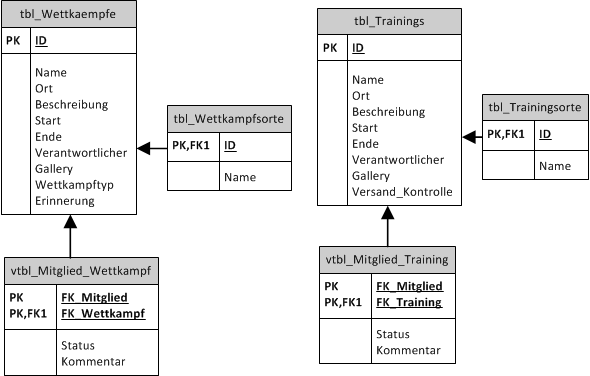
\includegraphics[scale=0.7]{images/visio/datenbankdiagramm_alt.png}
\caption{Datenbankdiagramm alt}
\label{fig:db_schema_alt}
\end{figure}

Das Datenbankdiagramm (siehe Abbildung \ref{fig:db_schema_alt}) zeigt einen kleinen Ausschnitt aus dem Datenbank Schema der Vergangenheit. Jeder Veranstaltungstyp hatte seine eigene Ortstabelle und seine eigene Verknüpfungstabelle für die Anmeldungen. Wenn man sich nun vorstellt, dass dieses Konstrukt für die fünf verschiedenen Typen vorhanden war, wird die grosse Anzahl der bereits für die Anmeldung notwendigen Tabellen offensichtlich. Nach dem \glossarmark{Refactoring} sah das Datenbankdiagramm (siehe Abbildung \ref{fig:db_schema_neu}) etwas einfacher aus. Die Orte und Anmeldungen sind nun in einer Tabelle und alle gemeinsamen Attribute wurden in der 'TerminObjekte' Tabelle gespeichert.

\begin{figure}[h]
\centering
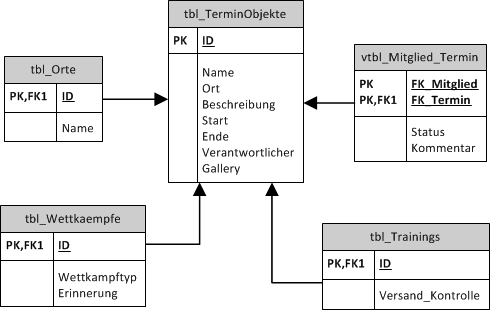
\includegraphics[scale=0.7]{images/visio/datenbankdiagramm_neu.png}
\caption{Datenbankdiagramm neu}
\label{fig:db_schema_neu}
\end{figure}

\FloatBarrier
Durch das \glossarmark{Refactoring} werden weniger SQL-Statements direkt in den Webseiten abgesetzt. Es wird vermehrt\footnote{Nur an Orten, an denen die Objekte innerhalb dieses Projektes angepasst wurden} mit Objekten gearbeitet. Ein Repository liefert die gewünschten Objekte zur Webseite, die Abfrage Logik ist somit zentralisiert. Das Repository arbeitet mit einer \glossarmark{Object Query Language} (\glossarmark{OQL}), bei welcher nicht über die Spalten der Tabelle Werte abgefragt werden, sondern über die Attribute des Objekts. Eine Änderung des Spaltennamens hat somit keine grössere Auswirkung als eine kleine Änderung in der Konfiguration der \glossarmark{Entity}.\\

Die Struktur sieht nach der Implementierung von Doctrine wie folgt aus:
\begin{itemize}
\item \glossarmark{Entity}: Attribute, Getter und Setter
\item \glossarmark{Entity}-Manager: speichert, löscht und lädt \glossarmark{Entities} oder gibt das Repository der \glossarmark{Entity} zurück
\item Repository: spezifische Abfrage-Logik
\item Services\footnote{Services werden nicht von Doctrine vorgegeben, wurden aber als eine weitere sogenannte Verarbeitungsschicht implementiert}: Business-Logik
\end{itemize}

\newpage
\subsubsection{Facts and Figures}
Das \glossarmark{Refactoring} war zwar sehr zeitaufwendig, hat jedoch bei einigen Implementationen die Komplexität stark reduziert, Zeitersparnisse eingebracht und wird auch in Zukunft vieles erleichtern.
\begin{itemize}
\item Testabdeckung: Das Testen stellte sich vorher als extrem schwierig heraus und ist nun mit den Kapselungen viel einfacher. Es konnte während des Projekts doch immerhin eine Testabdeckung von 11.1\% erreicht werden. Dieses Resultat wird natürlich noch sehr verfälscht durch Seiten und Funktionen, welche nicht Teil dieses Projekts waren.
\item Duplikate: Der Prozentsatz der duplizierten Linien konnte um fast 6\% reduziert werden, was etwa 4'000 Lines of code bedeutet.
\item Komplexität: Die Komplexität pro Klasse konnte von 40 auf 17 gesenkt werden.
\item Rule compliance: Die Rule compliance konnte um knapp 7\% gesteigert werden.
\item Issues: Über 3000 Issues, darunter alle kritischen und Blocker Issues, konnten behoben werden.
\end{itemize}


\subsection{Push-Nachrichten}
Das Versenden von Push-Nachrichten funktioniert bei iOS und Android ähnlich, jedoch sind die Vorbedingungen sehr unterschiedlich. Bei Android wird ein \glossarmark{API}-Key verwendet, welcher in der Google Developers Console erstellt werden kann. Dazu muss ein Projekt erstellt und '\glossarmark{Google Cloud Messaging for Android}' aktiviert werden. Nun kann ein neuer \glossarmark{API}-Key für die Verwendung im Backend generiert werden. Die Projektnummer ist zugleich die Sender ID und wird bei der Registrierung des produktiven Apps über Phonegap benötigt. (siehe dazu \cite{android_push_android} und \cite{devgirl_push_android})\\

Das Vorgehen bei iOS unterscheidet sich stark, als Erstes wird ein Zertifikat benötigt, da nur ein Server mit diesem Zertifikat Push-Nachrichten an den \glossarmark{APNS} senden darf. Es gibt ein Zertifikat für den Entwicklungsserver und ein weiteres für den produktiven Server. Über den Entwicklungsserver können nur verknüpfte\footnote{um die App auf einem Gerät zu testen, muss man es zuerst mit dem Developer Account verknüpfen} Geräte im Entwicklungsmodus erreicht werden. Zusätzlich muss für das Testen der Push-Nachrichten noch ein iOS App Development Provisioning Profile erstellt werden, welches dann auch mit dem Developer Account und den Test Geräten verknüpft wird. Bei der Erstellung der Zertifikate ist es wichtig, dass die App ID mit dem Projekt übereinstimmt, ansonsten kommen die Push-Nachrichten nicht an. Die Registrierung des produktiven Apps über Phonegap ist einfach und nicht projektspezifisch. (siehe dazu \cite{ios_push})\\

Nach der Registrierung des jeweiligen Services schickt die App den Geräteschlüssel mit der Mitglieder ID ans Backend, welches den Schlüssel mit der Verknüpfung zum Mitglied speichert. Nun ist der Schlüssel, für das gezielte Versenden von Push-Nachrichten vorhanden. (siehe Abbildung \ref{fig:push_notification_flow_reg} und \ref{fig:push_notification_flow_send})
\begin{figure}[ht]
\centering
\subfigure[Registration]{
  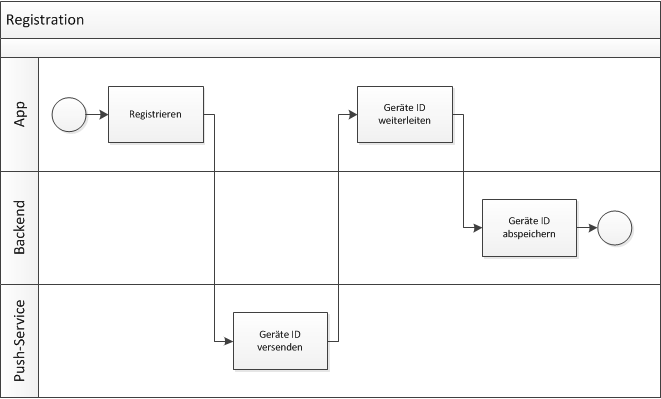
\includegraphics[scale=0.7]{images/visio/push_notification_flow_reg.png}
  \label{fig:push_notification_flow_reg}
}
\subfigure[Mitteilung versenden]{
  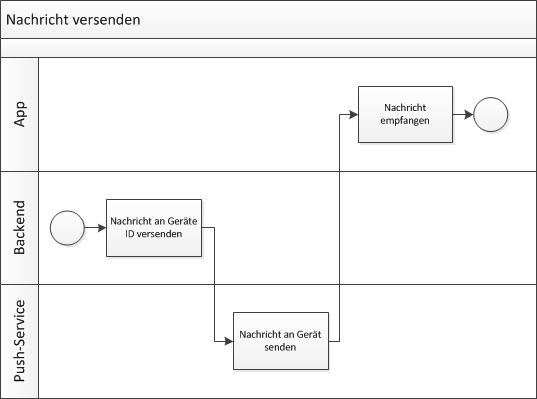
\includegraphics[scale=0.7]{images/visio/push_notification_flow_send.png}
  \label{fig:push_notification_flow_send}
}
\label{fig:app_settings}
\caption{Ablauf von Push-Nachrichten}
\end{figure}

\subsection{Resultierende Quellcode}
Dieses Projekt wurde auf einem bereits bestehenden Backend aufgebaut, alle Änderungen ab der Revision 3c54a42a698abdeee1779c71542786bd6707237b wurden innerhalb dieses Projekt getätigt. Für die Arbeiten im \glossarmark{Refactoring} wurden zwei neue Branches erstellt. Zum einen der 'refactoring' Branch, in welchem die Änderungen für die Datenmigration abgelegt wurden und zum anderen der 'jpa\_implementation' Branch, in welchem das eigentliche \glossarmark{Refactoring} durchgeführt wurde. In diesem Branch wurde gearbeitet bis der Stand produktionsreif war. Der 'jpa\_implementation' Branch wurde danach wieder in den 'master' Branch geführt.


\section{Mobile App}\label{impl_moblie_app}
In diesem Unterkapitel werden neben einem detailierten Aufbau der App, die unterschiedlichen Provisioning Prozesse und die Probleme bei der Umsetzung beschrieben.

\subsection{Aufbau}
Das Menü (siehe Abbildung \ref{fig:navigation}) der App wurde schlicht und sehr leicht erweiterbar gehalten. Die Einträge News, Vereine und Veranstaltungen sind für alle Benutzer sichtbar, wenn auch mit benutzerspezifischem Inhalt und Design. Der Link zu den Resultaten ist nur für angemeldete Benutzer verfügbar.

\begin{figure}[h]
\centering
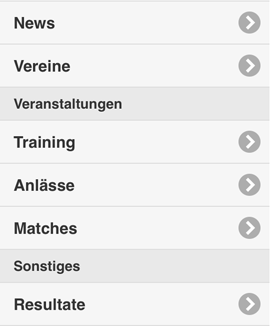
\includegraphics{images/app/navigation.png}
\caption{Navigation im App}
\label{fig:navigation}
\end{figure}

\FloatBarrier
\subsubsection{News}
Die News Seite (siehe Abbildung \ref{fig:app_news}) ist zugleich auch die Startseite, wenn die App geöffnet wird. Auf ihr werden die neusten drei Meldungen angezeigt. Der Aufbau ist wie auf der Homepage, die Elemente enthalten lediglich einen Einleitungstext. Erst nach dem Anwählen des Berichtes ist es möglich den ganzen Bericht zu lesen. Dies hat den einfachen Grund, dass die Berichte zum Teil sehr lang sind und dann die anderen Berichte verloren gehen. Bei angemeldeten Mitgliedern wird zusätzlich noch die nächste Veranstaltung angezeigt, damit man sich sofort an- bzw. abmelden und wichtige Informationen nachschlagen kann.

\begin{figure}[h]
\centering

\includegraphics[scale=0.5]{images/app/news.png}
\caption{News Seite}
\label{fig:app_news}
\end{figure}

\FloatBarrier
\subsubsection{Vereine}
Die Vereine Seite (siehe Abbildung \ref{fig:app_vereine})  listet alle Vereine und Riegen der Turner Familie Grafstal auf. Nach der Auswahl einer Riege, erhält man zusätzliche Informationen, wie zum Beispiel die Trainingszeiten. Diese Seite enthält vor allem Informationen für die Öffentlichkeit oder ist ein Nachschlagewerk für Mitglieder.


\begin{figure}[h]
\centering
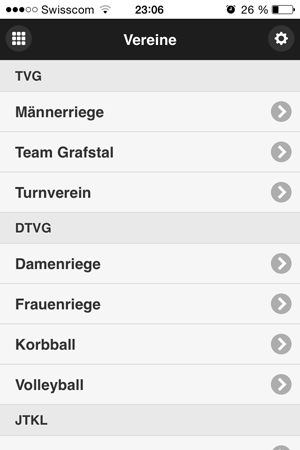
\includegraphics[scale=0.5]{images/app/vereine.png}
\caption{Vereinsseite}
\label{fig:app_vereine}
\end{figure}

\newpage
\FloatBarrier
\subsubsection{Veranstaltungen}
Die drei Veranstaltungsseiten sind alle gleich aufgebaut (siehe Abbildung \ref{fig:app_trainings}), sie zeigen die aktuellen Elemente mit Name, Datum, Zeit, Ort und Verantwortlichen. Falls der Benutzer angemeldet ist, wird durch Farbe angezeigt, ob er sich angemeldet (grün), abgemeldet (rot) oder nichts dergleichen (grau) hat.
\begin{figure}[ht]
\centering
\subfigure[Anlässe (nicht angemeldet)]{
  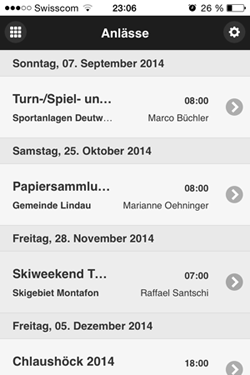
\includegraphics[scale=0.5]{images/app/events.png}
  \label{fig:app_events}
}
\subfigure[Trainings (angemeldet)]{
  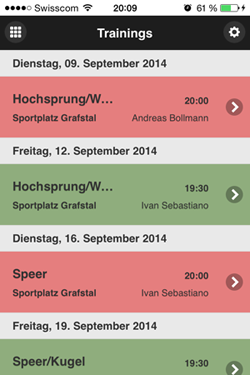
\includegraphics[scale=0.5]{images/app/trainings.png}
  \label{fig:app_trainings}
}
\label{fig:app_singinobjects}
\caption{Veranstaltungen}
\end{figure}

Wenn auf eine Veranstaltung geklickt wird, öffnet sich eine Detailansicht (siehe Abbildung \ref{fig:app_detail_event}). In dieser Ansicht sind weitere Information verfügbar, es kann sich an- und abgemelden werden und man gelangt zu den Fahrgemeinschaften. Die Information, wer sich angemeldet hat, sehen nur angemeldete Benutzer.

\begin{figure}[h]
\centering
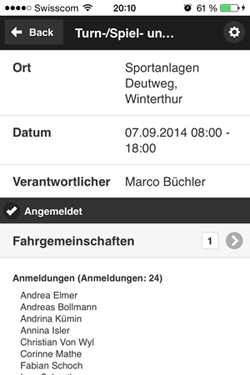
\includegraphics[scale=0.5]{images/app/event_detail.png}
\caption{Anlass Details}
\label{fig:app_detail_event}
\end{figure}

\newpage
\FloatBarrier
\subsubsection{Fahrgemeinschaften}
Bei jeder Veranstaltung können Fahrgemeinschaften erstellt werden, welche dann in der Übersicht (siehe Abbildung \ref{fig:app_carpools}) angezeigt werden. Es ist der Namen, der Fahrer und dessen Wohnort ersichtlich. Zusätzlich ist erkennbar, wie viele Plätze noch frei sind oder ob man bereits angemeldet ist. In der Detailansicht (siehe Abbildung \ref{fig:app_carpool_detail}) gibt es die Möglichkeit sich anzumelden und es erscheint eine Liste der Mitfahrenden.
\begin{figure}[ht]
\centering
\subfigure[Fahrgemeinschaften]{
  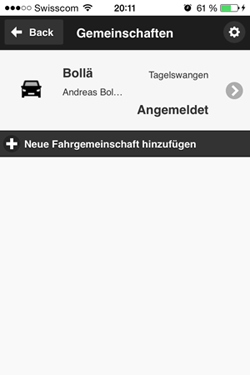
\includegraphics[scale=0.5]{images/app/carpools.png}
  \label{fig:app_carpools}
}
\subfigure[Fahrgemeinschaft Detail]{
  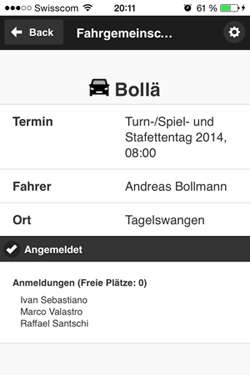
\includegraphics[scale=0.5]{images/app/carpool_detail.png}
  \label{fig:app_carpool_detail}
}
\label{fig:app_carpool_page}
\caption{Veranstaltungen}
\end{figure}

Im Formular (siehe Abbildung \ref{fig:app_add_carpool}) für die Erstellung einer neuen Fahrgemeinschaft muss ein Name und der Typ der Gemeinschaft angegeben werden, nur wenn es eine 'Car'-Fahrgemeinschaft ist, muss man die freien Plätze angeben.

\begin{figure}[h]
\centering
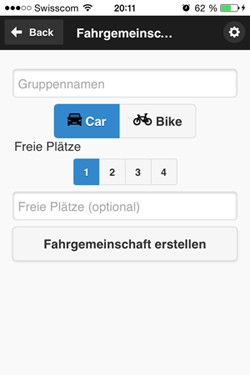
\includegraphics[scale=0.5]{images/app/add_carpool.png}
\caption{Fahrgemeinschaft erstellen}
\label{fig:app_add_carpool}
\end{figure}


\newpage
\FloatBarrier
\subsubsection{Resultate}
Unter Resultate (siehe Abbildung \ref{fig:app_results}) finden angemeldete Benutzer ihre Bestleistungen und die Resultate für die \glossarmark{Büchsenliste}.
\begin{figure}[h]
\centering
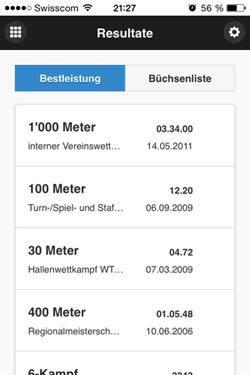
\includegraphics[scale=0.5]{images/app/results.png}
\caption{Resultate Seite}
\label{fig:app_results}
\end{figure}


\FloatBarrier
\subsubsection{Einstellungen}
In den Einstellungen kann sich der Benutzer nicht nur einloggen (siehe Abbildung \ref{fig:app_login}), sondern auch wählen, für welche Riege er die Matches, Anlässe und Trainings sehen möchte (siehe Abbildung \ref{fig:app_riege_setting}). Diese Filter werden dann auf die Veranstaltungsübersichtseiten angewendet.
\begin{figure}[ht]
\centering
\subfigure[Login Formular]{
  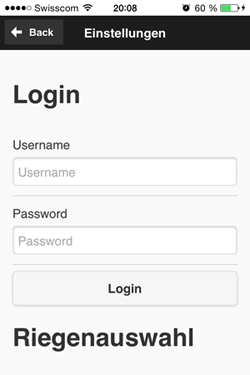
\includegraphics[scale=0.5]{images/app/settings1.png}
  \label{fig:app_login}
}
\subfigure[Riegen Einstellungen]{
  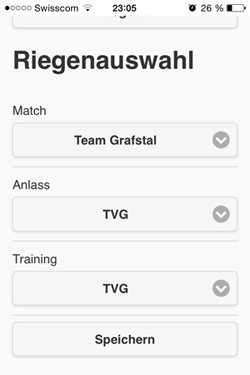
\includegraphics[scale=0.5]{images/app/settings2.png}
  \label{fig:app_riege_setting}
}
\label{fig:app_settings}
\caption{Einstellungen}
\end{figure}

\newpage
\FloatBarrier
\subsection{Javascript Funktionen}
Die Javascript Funktionen wurden möglichst generisch gewählt, damit sie an verschiedenen Orten wiederverwendet werden können. Mit diesem Ansatz ist bei den verschiedenen Veranstaltungsseiten wenig Code nötig gewesen. Es war auch einfach, die nächste bevorstehende Veranstaltung auf der Startseite gleich, wie auf den anderen Seiten, anzuzeigen. Die App kommt dadurch mit knapp 2'000 Zeilen Code aus. Die Funktionen wurden in unterschiedliche Files geschrieben, welche nach ihrem Zweck benannt wurden.
\begin{itemize}
\item carpool.js: an- und abmelden bei Fahrgemeinschaften, anzeigen von Fahrgemeinschaften
\item help.js:  Datum formatieren,  Listen-Elemente erstellen, Navigationselemente
\item index.js: initialisieren der Push-Benachrichtigungen
\item news.js: Berichte laden
\item result.js: Resultate anzeigen
\item settings.js: Dropwdowns initialisieren, an- und abmelden, Riegenfilter setzen
\item signinObject.js: Veranstaltungen laden, Veranstaltungsdetails anzeigen, an- und abmelden bei Veranstaltungen 
\end{itemize}

\subsection{Login}
Da das Backend nur über eine HTTP-Verbindung verfügte und die Anmeldedaten nicht im \glossarmark{localStorage}  gespeichert werden sollten, wurde darauf verzichtet, die Anmeldedaten bei jeder Anfrage an das Backend mitzusenden. Bei der Anmeldung wird die Mitglieder-ID gespeichert und bei einer Anfrage mitgeteilt. In einem späteren Projekt sollte diese Lösung durch eine \glossarmark{Session-ID} in Verbindung mit einer HTTPS-Verbindung abgelöst werden.

\subsection{Provisioning Prozesse}
Die Entwicklung der App ist das Eine, die Bereitstellung zum Download das Andere. Phonegap hilft beim Provisioning vor allem bei Android. Es erstellt, richtig konfiguriert, ein signiertes APK-Paket, welches in der Google Play Developer Console hochgeladen werden kann. Zuerst muss jedoch einen Developer Account eröffnet werden. Anschliessend können die Beschreibung und die Screenshots für die App hochgeladen werden. Dies dauert nur wenige Minuten, eine Stunde nach dem Absenden findet man seine App in Google Play. Es empfiehlt sich, die App noch mit einer Absender-ID zu verknüpfen, damit man Statistiken über die Downloadzahlen ansehen kann. (siehe dazu auch \cite{android_prov})

Bei Apple sieht das etwas anders aus: Phonegap kann kein Paket erstellen, es erstellt lediglich das Projekt. Das Projekt muss dann in XCode geöffnet und von dort aus das eigentliche Paket erstellet werden. Auch hier wird ein Developer Account vorausgesetzt, diesen besitzt man wahrscheindlich bereits, da ohne ihn nicht auf realen Geräten getestet werden kann. Zusätzlich muss ein Distribution Certificate erstellt und in XCode hingezufügt werden. Danach müssen in iTunes Connect noch einige Angaben zu den Inhalten der App gemacht werden. Des Weiteren werden Review Informationen verlangt, welche aus einem Test Benutzer und Informationen zur Entwicklung bestehen. Erst wenn die App erfasst wurde, kann in XCode ein Archiv erstellt und dieses direkt zu iTunes Connect hochgeladen werden. Nun werden bereits die ersten Tests durchgeführt, beispielsweise ob die Versionsnummern übereinstimmen und ob für jedes unterstützte Gerät Screenshots erfasst wurden. Falls dies nicht der Fall ist, wird die App abgelehnt und die Dinge müssen zuerst behoben werden. An diesem Punkt beginnt das Warten - die durchschnittliche Review-Zeit beträgt 8 Tage. (siehe dazu auch \cite{apple_prov_apple} und \cite{apple_prov_ralf})

\subsection{Probleme}
Die Entwicklung für verschiedenen Plattformen war nicht immer einfach. Es kann zwar der gleiche Code verwendet werden, jedoch wird dieser zum Teil anders interpretiert. Bei iOS stellte zum Beispiel die Datum Konvertierung von Daten aus \glossarmark{PHP} in Javascript ein Problem dar. Die Daten mussten aufgesplittet werden und in Javascript ein neues Datum Objekt mit den einzelnen Teilen erstellt werden. Des Weiteren wurde unter Android der Löschaufruf für Fahrgemeinschaften gepuffert. Die App zeigte zwar an, dass die Fahrgemeinschaft gelöscht worden sei, doch es wurde nie ein Löschauftrag an das Backend gesendet. Dieser Fehler wurde bei jQuery raportiert (siehe \cite{bug_jquery}) und mittels eines Workarounds umgangen. Ein weiterer Fehler (siehe \cite{bug_jquery_mobile}) wurde in jQuery Mobile gefunden, es gab hier Probleme mit der Navigation, wenn die grafischen Übergange von jQuery Mobile abgeschaltet wurden. Dieser Fehler konnte jedoch auch mit einem Workaround umgangen werden.
